\documentclass[dvisvgm,tikz,border=4pt]{standalone}\usepackage{amsmath,amssymb}
\usetikzlibrary{arrows.meta,decorations.markings,backgrounds,cd,calc}
\colorlet{c1}{blue!70!black}\colorlet{c2}{red!70!black}\colorlet{c3}{green!45!black}
\tikzset{
 ->-/.style={decoration={markings,mark=at position .55 with {\arrow{Stealth[length=2.4mm]}}},postaction={decorate}},
 ->>-/.style={decoration={markings,mark=at position .5 with {\arrow{Stealth[length=2.4mm]}},mark=at position .6 with {\arrow{Stealth[length=2.4mm]}}},postaction={decorate}},
 every picture/.append style={show background rectangle, background rectangle/.style={fill=white}}
}

\begin{document}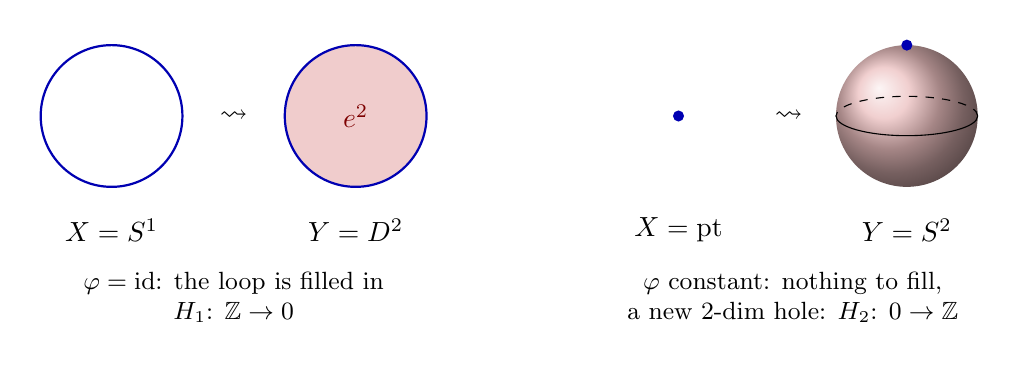
\begin{tikzpicture}
% example 1: S^1 + e^2 = D^2
\begin{scope}
\draw[thick,c1] (0,0) circle(0.9);
\node at (0,-1.45){$X=S^1$};
\node at (1.55,0){$\leadsto$};
\begin{scope}[xshift=3.1cm]
\fill[c2!20] (0,0) circle(0.9); \draw[thick,c1] (0,0) circle(0.9);
\node[c2!70!black] at (0,0){$e^2$};
\node at (0,-1.45){$Y=D^2$};
\end{scope}
\node[align=center,font=\small] at (1.55,-2.3){$\varphi=\mathrm{id}$: the loop is filled in\\ $H_1$: $\mathbb{Z}\to0$};
\end{scope}
% example 2: point + e^2 = S^2
\begin{scope}[xshift=7.2cm]
\fill[c1] (0,0) circle(2pt);
\node at (0,-1.45){$X=\mathrm{pt}$};
\node at (1.4,0){$\leadsto$};
\begin{scope}[xshift=2.9cm]
\shade[ball color=c2!25] (0,0) circle(0.9);
\draw (-0.9,0) arc(180:360:0.9 and 0.25);
\draw[dashed] (0.9,0) arc(0:180:0.9 and 0.25);
\fill[c1] (0,0.9) circle(2pt);
\node at (0,-1.45){$Y=S^2$};
\end{scope}
\node[align=center,font=\small] at (1.45,-2.3){$\varphi$ constant: nothing to fill,\\ a new 2-dim hole: $H_2$: $0\to\mathbb{Z}$};
\end{scope}
\end{tikzpicture}\end{document}
